We notice that there is a common subexpression between the trees; we can express the optimisation that results from only calculating this once by turning our trees into a DAG, as follows:

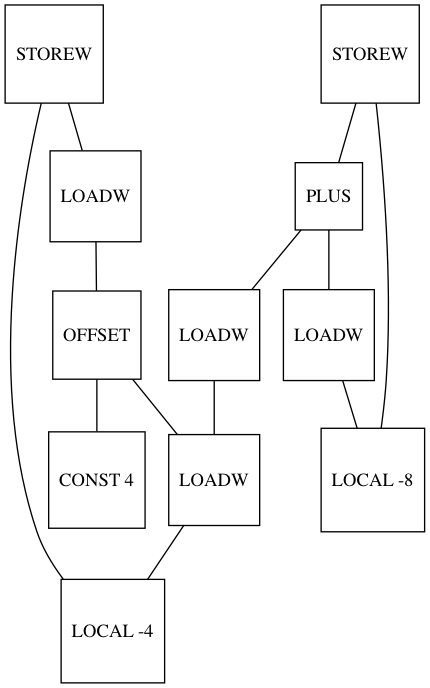
\includegraphics[width=\textwidth]{ex4.png}

(note that although we eliminated the common \texttt{LOCAL} subtrees, this does not actually improve the object code generated, as those values are handled by ARM's adressing modes).

This optimisation creates the following code, that no longer recalculates [fp, \#-4].

\begin{lstlisting}
ldr r0, [fp, #-4]
ldr r1, [r0]
add r1, r1, [fp, #-8]
str r1, [fp, #-8]
ldr r1, [r0, #4]
str r1, [fp, #-4]
\end{lstlisting}
